%%
%% This is file `sample-sigconf.tex',
%% generated with the docstrip utility.
%%
%% The original source files were:
%%
%% samples.dtx  (with options: `sigconf')
%% 
%% IMPORTANT NOTICE:
%% 
%% For the copyright see the source file.
%% 
%% Any modified versions of this file must be renamed
%% with new filenames distinct from sample-sigconf.tex.
%% 
%% For distribution of the original source see the terms
%% for copying and modification in the file samples.dtx.
%% 
%% This generated file may be distributed as long as the
%% original source files, as listed above, are part of the
%% same distribution. (The sources need not necessarily be
%% in the same archive or directory.)
%%
%% The first command in your LaTeX source must be the \documentclass command.
\documentclass[sigconf]{acmart}
\usepackage[spanish]{babel}
\usepackage[utf8]{inputenc}
\usepackage{lmodern}
\usepackage{tabularx}
\usepackage{listings}




%%
%% \BibTeX command to typeset BibTeX logo in the docs
\AtBeginDocument{%
  \providecommand\BibTeX{{%
    \normalfont B\kern-0.5em{\scshape i\kern-0.25em b}\kern-0.8em\TeX}}}





%%
%% end of the preamble, start of the body of the document source.
\begin{document}

%%
%% The "title" command has an optional parameter,
%% allowing the author to define a "short title" to be used in page headers.
\title{Práctica 1}

%%
%% The "author" command and its associated commands are used to define
%% the authors and their affiliations.
%% Of note is the shared affiliation of the first two authors, and the
%% "authornote" and "authornotemark" commands
%% used to denote shared contribution to the research.
\author{Jorge Humberto Sierra Florido}
\email{2123065656@cua.uam.mx}
\affiliation{
  \institution{UAM Cuajimalpa \\ Ingeniería en Computación}
  \city{Ciudad de México}
  \country{México}
}

\author{María de Jesús Sánchez Zepeda}
\email{2153068423@cua.uam.mx}
\affiliation{
  \institution{UAM Cuajimalpa\\ Ingeniería en Computación}
  \city{Ciudad de México}
  \country{México}
}

%%
%% The abstract is a short summary of the work to be presented in the
%% article.
\begin{abstract}
  Aqu{\'i} va el abstract de la pr{\'a}ctica...
\end{abstract}

%%
%% This command processes the author and affiliation and title
%% information and builds the first part of the formatted document.
\maketitle

\section{Introducción}

En el análisis de datos es importante la limpieza de los datos previos a realizar modelos predictivos con ellos. Con limpieza nos referimos al tratamiento de los datos faltantes con el fin de no inducir un sesgo en el modelo.

Para encontrar relaciones entre dos variables continuas definidas en la misma población se puede utilizar el coeficiente de correlación y la regresión líneal. En está práctica se tienen dos conjuntos de datos de diferentes tamaños a los cuáles se les desea encontrar un modelo una ecuación que modele la relación entre variables determinadas.Para ello se limpiarán los datos de cada conjunto, posteriormente se generaran los diagramas de dispersión que nos ayudan a identificar los \textit{outloaders}. Después se realizará una regresión lineal para posteriormente evaluar cada modelo, para ello se cálculará la eficiencia del modelo generado y el grado de error que contiene.

Texto introductorio al tema en que se enfoca la pr{\'a}ctica y lo que se desarrollar{\'a} en ella. Se debe escribir un texto que introduzca el tema de la 
pr{\'a}ctica, definici{\'o}n del problema, los objetivos, motivaci{\'o}n,  y resultados esperados.

\section{Conceptos previos}

Escribir conceptos te{\'o}ricos empleados en el desarrollo de la pr{\'a}ctica (f{\'o}rmulas matem{\'a}ticas, por ejemplo). Es un tipo de secci{\'o}n con todos los conceptos te{\'o}ricos empleados.

\section{Metodología}

Se analizaron los datasets usando el lenguaje de programación R\footnote{R es un lenguaje orientado a computo estadístico y de gráficas, \url{https://www.r-project.org/} } y el IDE R studio. a fin de generar los resúmenes estadísticos y gráficas requeridas, esto tras limpiarlos de información faltante.

Posteriormente se procedió al análisis de la información usando Python, ayudándonos de Scikit-Learn , Pandas y Numpy.
Se requirió investigar la función LinearRegression, para aplicarla a los datasets y generar los modelos

Finalmente se evaluaran los modelos y se compararan la regresion lineal normal y la ponderada.

\section{Resultados}

Se inicio la practica revisando los datasets proporcionados, estos corresponden a los datos de temperatura y salinidad medidas, así como las características de algunos vehículos. 

El primer paso fue cargar los datos en R a fin de poder analizar los datasets. para esta carga se usaron las instrucciones del Código \ref{lst:cargaDatos}

\begin{lstlisting}[caption=lectura de los datos,breaklines,label=lst:cargaDatos]
data = read.csv("water.csv", header=TRUE)
data2 = read.table("mtcars.txt", header=TRUE , sep = " ")
\end{lstlisting}

Una vez cargada la información se procedió a obtener el resumen de la misma con la siguiente instrucción del Código \ref{lst:resumen1}, generando la salida mostrada en la Tabla \ref{tab:Tabla1}

\begin{lstlisting}[caption=Resumen de los datos,breaklines,label=lst:resumen1]
summary(data)
\end{lstlisting}

\begin{table}
	\begin{tabularx}{\columnwidth}{|X|X|X|X|}
		\hline
		\multicolumn{2}{|c|}{ TdegC } & \multicolumn{2}{|c|}{ Salnty }  \\
		\hline
		Min. & 1.44  & Min. & 28.43 \\
		\hline
		1st Qu.& 7.68 &1st Qu.&33.49 \\
		\hline
		Median &10.06  & Median & 33.86   \\
		\hline
		Mean & 10.80 & Mean & 33.84\\
		\hline
		3rd Qu.&13.88 & 3rd Qu. & 34.20\\
		\hline
		Max. & 31.14 & Max.& 37.03  \\
		\hline
		NA's & 10963 & NA's  & 47354\\
		\hline
	\end{tabularx}
	\caption{\label{tab:Tabla1}Resumen de el dataset water.csv}
\end{table}

En la Tabla \ref{tab:Tabla1} se observaron 10963 registros vacíos en el campo de temperatura y 47354 en la salinidad.
Se eligió como alternativa dejar los elementos con campos NA, remplazándolos por su Mediana, esto para no afectar el dataset. Este remplazo se realizo usando el Código \ref{lst:remplazo1}

\begin{lstlisting}[caption=Código de emplazo de los NA,breaklines,label=lst:remplazo1]
	data$Salnty[is.na(data$Salnty)] = 33.86
	data$TdegC[is.na(data$TdegC)] = 10.06
\end{lstlisting}

El nuevo resumen genero la Tabla \ref{label}. Donde se observan cambios mínimos.

\begin{table}
	\begin{tabularx}{\columnwidth}{|X|X|X|X|}
		\hline
		\multicolumn{2}{|c|}{ TdegC } & \multicolumn{2}{|c|}{ Salnty }  \\
		\hline
		Min. & 1.44  & Min. & 28.43 \\
		\hline
		1st Qu.& 7.72 &1st Qu.&33.50 \\
		\hline
		Median &10.06  & Median & 33.86   \\
		\hline
		Mean & 10.79 & Mean & 33.84\\
		\hline
		3rd Qu.&13.83 & 3rd Qu. & 34.18\\
		\hline
		Max. & 31.14 & Max.& 37.03  \\
		\hline
	\end{tabularx}
	\caption{\label{tab:Tabla2}Resumen limpio de el dataset water.csv}
\end{table}

Respecto a los datos 

Imagen de prueba

% TODO: \usepackage{graphicx} required
\begin{figure}
	\centering
	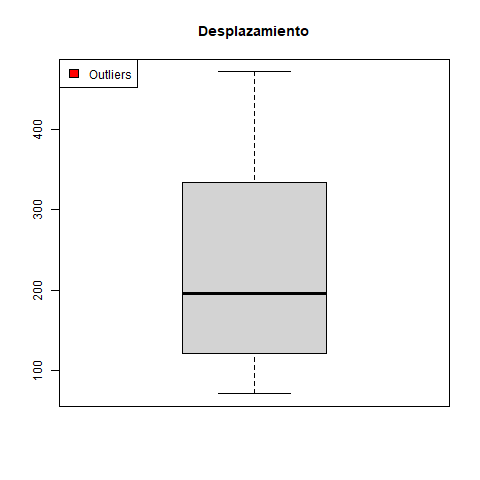
\includegraphics[width=0.7\linewidth]{img/dispBoxplot}
	\caption{Esto es una imagen de ejemplo}
	\label{fig:dispboxplot}
\end{figure}



\section{Conclusiones y reflexiones}

Conclusiones generales de la pr{\'a}ctica. A\~nadir una reflexi{\'o}n anal{\'i}tica por cada miembro del equipo.

%%
%% The next two lines define the bibliography style to be used, and
%% the bibliography file.
\bibliographystyle{ACM-Reference-Format}
\bibliography{references}


\end{document}
\endinput
%%
%% End of file `sample-sigconf.tex'.
